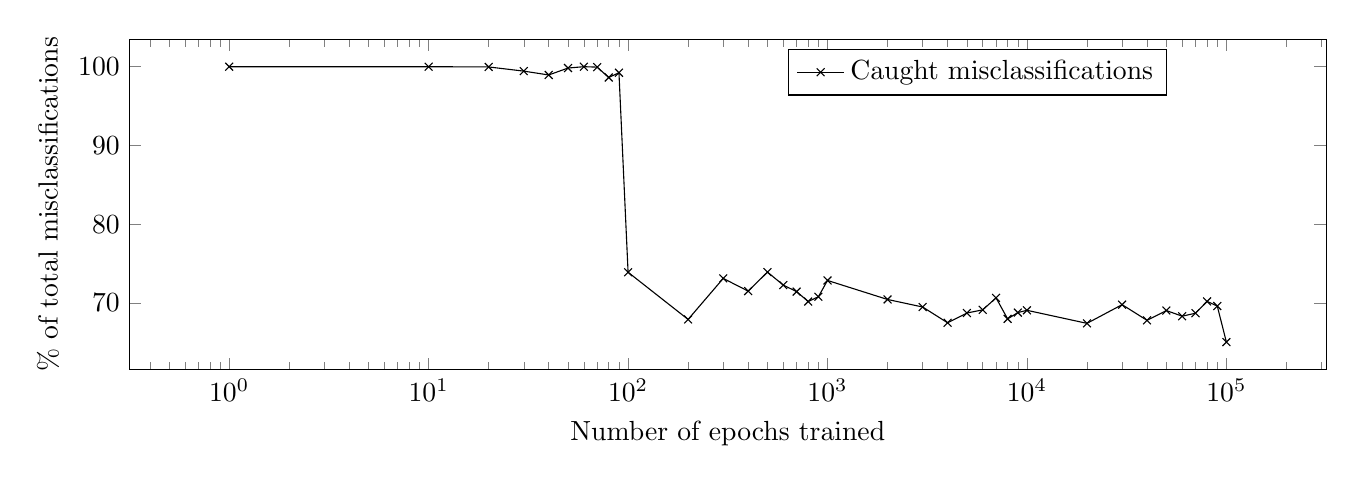
\begin{tikzpicture}
\begin{semilogxaxis}[
xlabel={Number of epochs trained},
ylabel={\% of total misclassifications},
x=1.1cm,
y=1.0mm, 
legend style={at={(0.55,0.9)},anchor=west}]

\addplot[color=black,mark=x] coordinates {
	(1, 100.000000)
	(10, 100.000000)
	(20, 99.968513)
	(30, 99.438622)
	(40, 98.948822)
	(50, 99.831619)
	(60, 100.000000)
	(70, 99.946243)
	(80, 98.629845)
	(90, 99.235352)
	(100, 73.896217)
	(200, 67.904327)
	(300, 73.114166)
	(400, 71.500191)
	(500, 73.917786)
	(600, 72.264412)
	(700, 71.438644)
	(800, 70.175438)
	(900, 70.787399)
	(1000, 72.854225)
	(2000, 70.439842)
	(3000, 69.480080)
	(4000, 67.477409)
	(5000, 68.717560)
	(6000, 69.121811)
	(7000, 70.645164)
	(8000, 67.972473)
	(9000, 68.772896)
	(10000, 69.063011)
	(20000, 67.405907)
	(30000, 69.780220)
	(40000, 67.787842)
	(50000, 69.032257)
	(60000, 68.315018)
	(70000, 68.693977)
	(80000, 70.194382)
	(90000, 69.604439)
	(100000, 65.025040)
};


\legend{Caught misclassifications, Uncaught misclassifications}
\end{semilogxaxis}%
\end{tikzpicture}%